%!TEX root = ../memoire.tex

\chapter{GenDR}\label{chapgendr}

GenDR (Generic Deep Realizer \citep{lareau18}) est un réalisateur profond multilingue.C'est un héritier de MARQUIS dans le sens où il utilise une architecture similaire pour la réalisation. C'est une plateforme pour la modélisation de l'interface sémantique-syntaxe. Ainsi, GenDR se démarque de MARQUIS par la couverture beaucoup plus importante qu'il offre en termes de locutions et collocations. Cette couverture lexicale a été fait par Lareau et Lambrey \cite{LambreyImplementationcollocationspour2017}, \cite{lambrey15}.

%%%%%%%%%%%%%%%%%%%%%%%%%%%%%%%%%%%%%%%%%%%%%%%%%%%%%%%
% --------- A R C H I T E C T U R E  GENDR  ---
%%%%%%%%%%%%%%%%%%%%%%%%%%%%%%%%%%%%%%%%%%%%%%%%%%%%%%%
\section{Architecture de GenDR}

Dans la section suivante, nous allons brièvement présenter MATE, la plateforme qui permet à GenDR de fonctionner. Puis nous allons brièvement décrire la composante multilingue de GenDR.

\subsection{MATE}

GenDR roule sur MATE \citep{BohnetDevelopmentEnvironmentMTTbased2000}, \citep{BohnetOpensourcegraph2010},\citep{Lareau2007TowardsAG}

\draft{Les transducteurs de graphes sont utilisés dans plusieurs applications en TAL, notamment en GAT (Bohnet et Wanner, 2010). MATE est un transducteur de graphes libre conçu par Bernd Bohnet (Bohnet, 2006; Bohnet, Langjahr, et Wanner, 2000; Bohnet, Lareau, Wanner, et al., 2007; Bohnet et Wanner, 2010) conçu à la base pour modéliser l’approche multistratale de la TST. Il manipule divers types de graphes et construit, à partir d’un graphe source, un graphe correspondant d’un niveau supérieur, sans modifier la structure de départ.
MATE fournit également une plateforme de développement et de maintien de générateurs de texte employant la TST (Bohnet et al., 2000). Pour passer d’un graphe à l’autre, MATE applique des règles et forme le graphe de sortie par un procédé d’unification. Nous ne rentrerons pas dans les détails techniques du fonctionnement de MATE et nous encourageons le lecteur intéressé à se référer à (Bohnet et Wanner, 2010).

En plus d’être un transducteur de graphe, MATE est aussi une plateforme de développement et de maintien de ressources à large couverture. (Bohnet et al., 2000) indiquent que MATE permet d’écrire, modifier et tester à la fois des dictionnaires et des grammaires. Il permet une structuration hiérarchique de ces ressources grâce à un système de classes. Chaque type de ressource possède son propre éditeur. MATE permet aussi de créer des structures à différents niveaux d’abstraction grâce à un éditeur dédié. MATE offre la possibilité de visualiser les différents graphes et fournit un inspecteur pour examiner le processus de correspondance lors de l’application des règles. L’inspecteur montre les correspondances établies entre les noeuds, l’instanciation des variables des règles appliquées et une trace de toutes les opérations effectuées pendant la compilation, ce qui favorise le développement et le maintien de larges grammaires. Nous allons maintenant nous attarder sur l’encodage des dictionnaires et des grammaires dans MATE.}

\subsection{Structures d'entrées et de sorties}\label{entree-sortie}
L'input de GenDR est des structures sémantiques de type TST. Il s'agit de graphes sémantiques où les prédicats sont liés à leurs arguments par des relations étiquettées avec des chiffres indiquant la position de l'argument. L'une des unités sémantiques doit être identifiée comme étant la plus saillante de l'énoncé. Il s'agit du noeud dominant de la phrase. Il sera mappé en tant que la racine syntaxique.

Voici à quoi ressemble l'input :
\begin{lstlisting}[language=XML, caption = Input sémantique, label=input]
structure Sem debt {
S {
owe {
tense=PRES
1-> Paul {class=proper_noun}
2-> "\$500K" {class=amount}
3-> bank {number=SG definiteness=DEF}}
main-> owe}}
\end{lstlisting}

Mais pour simplifier la chose, nous montrerons une version graphique: insérer une structure sémantique
\begin{figure}[htb]
	\centering
	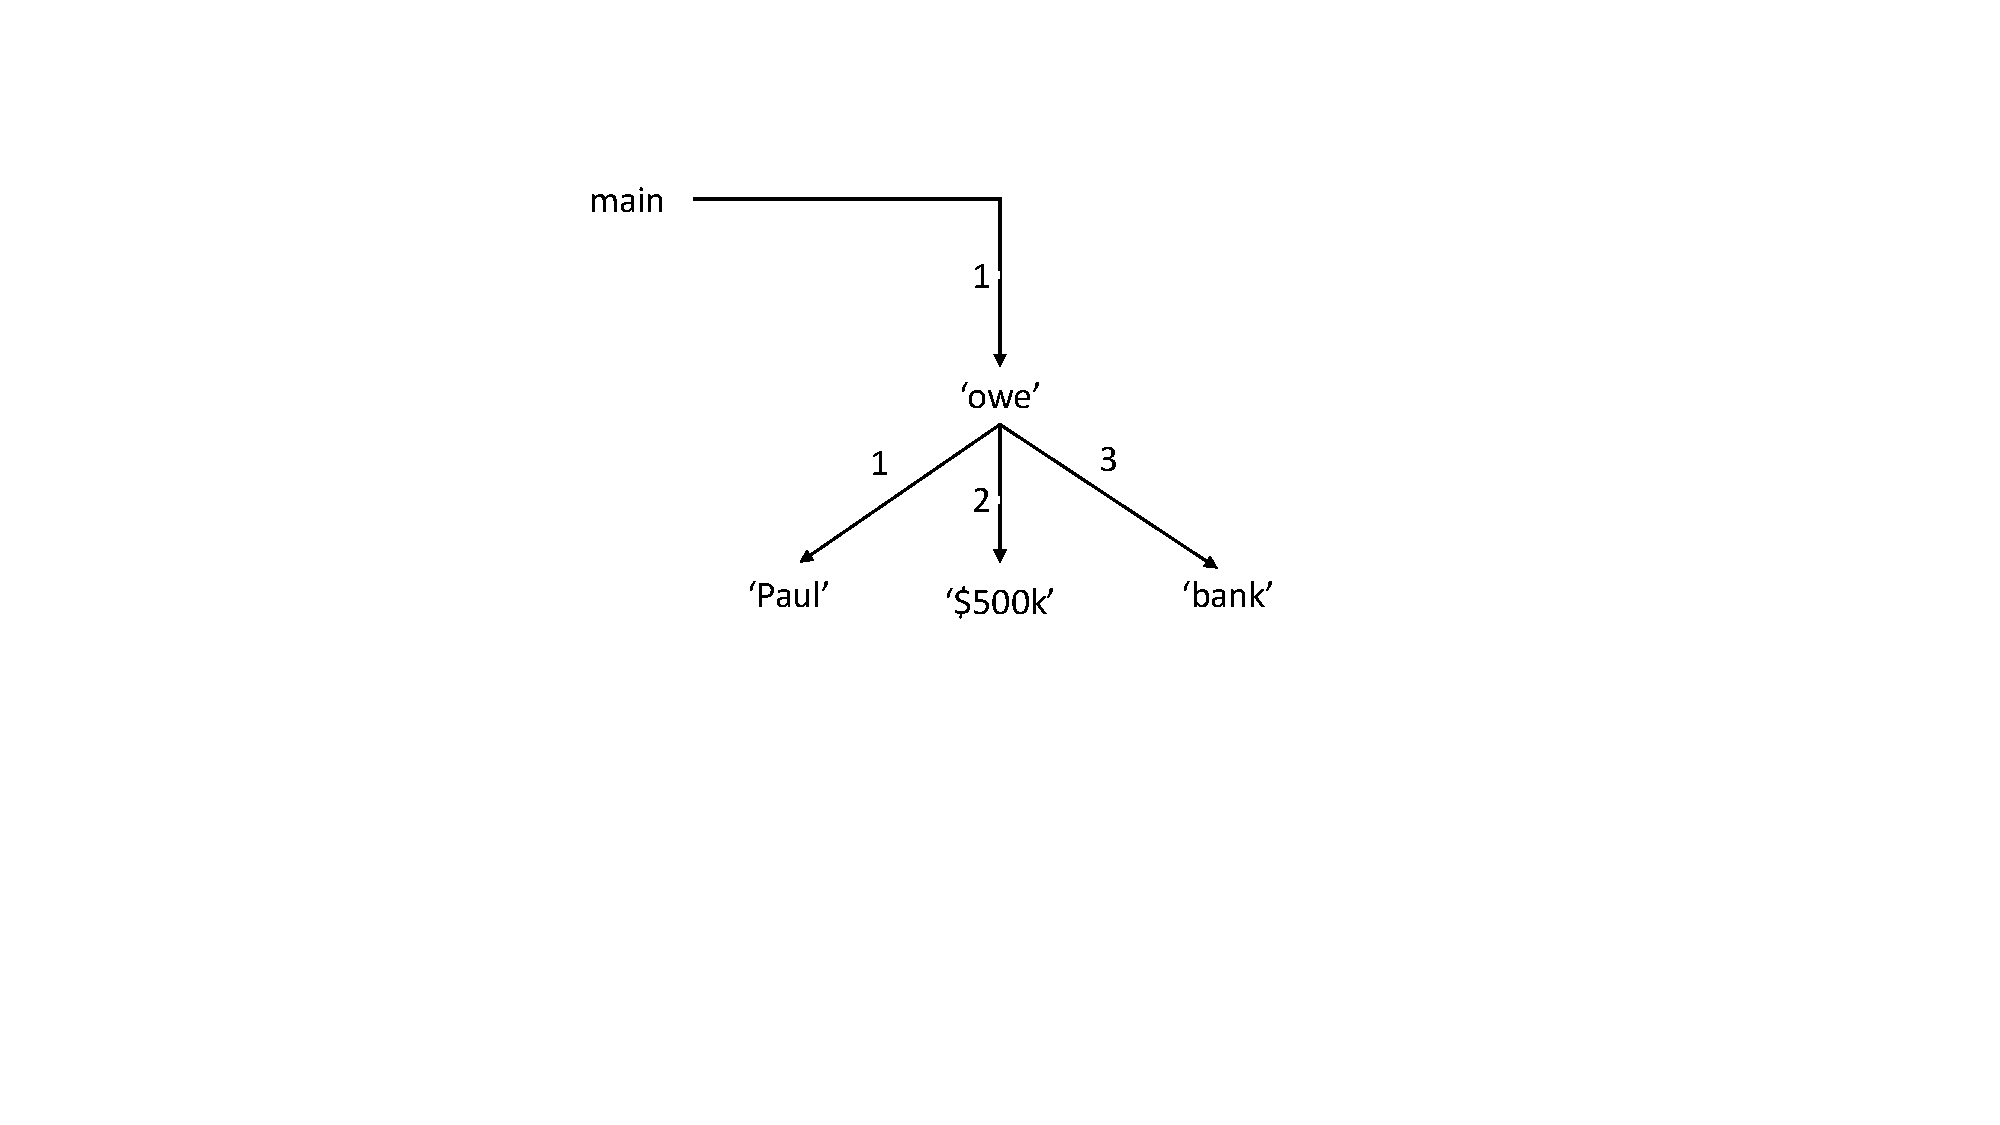
\includegraphics[width=1\textwidth, trim = {0cm 0cm 0cm 0cm},clip]{ch3/figs/owe_sem.pdf}
	\caption{Graphe sémantique en visuel}
	\label{fig:graphesem}
\end{figure}

L'output de ce système consiste en un ensemble de structures de dépendances syntaxiques de surface. Ainsi, avec l'input sémantique en \ref{input} le réalisateur génère les six structures suivantes. 

\draft{faire les 2 structures en version graphique et montrer les informations qu'ils portent sur leur code}

Toutefois, afin de générer le texte final désiré à partir de l'input, il faudra passer par un réalisateur de surface. GenDR ne traite pas l'interface morpho-syntaxique et ne linéarise pas le texte. C'est dans ces contextes, que les réalisateurs de surface mentionnées précédement entrent en jeu. GenDR met plutôt l'accent sur les tâches plus profondes de la réalisation, notamment l'arborisation et la lexicalisation.

\subsection{Aspect multilingue}
Tel que mentionné, GenDR est une grammaire multilingue. Les règles grammaticales de base sont directement héritée de MARQUIS(citation) qui pouvait réaliser du texte en : catalan, anglais, français, polonais, portugais et espagnol. Ils n'ont gardé que les règles de base qui décrivent des phénomènes langagiers de base: lexicalisation simple, complementation, modification,etc. Ces règles forment le noyau du système et sont partagées (la majorité) par l'ensemble des langues du systèmes. Les règles spécifiques aux langues modélisent des phénomènes comme la sélection des auxiliaires, les déterminants, etc.

Le mapping entre les graphes sémantiques et les structures syntaxiques de surface se fait en deux étapes. Ces deux étapes sont effectuées par l'entremise de deux modules de règles différents opérant les interfaces respectives. Le module sémantique mappe les graphes sémantiques aux structures syntaxiques profondes correspondantes (Melcuk,2013), tandis que le module syntaxique mappe les structures syntaxiques profondes aux strucutres syntaxiques de surface. Cette architecture stratifiée est directement inspirée de la théorie Sens-Texte (melcuk et compagnie).

Ainsi le module sémantique contient 21 règles dont la plupart sont héritées de MARQUIS et 132 règles de lexicalisation \citep{LambreyImplementationcollocationspour2017}. Pour sa part, le module syntaxique contient nettement moins de règles. 20 règles dont 12 partagées entre les langues. Chaque règle modélise un phénomène langagier sur quoi la grammaire compte sur la richesse des dictionnaires.

%%%%%%%%%%%%%%%%%%%%%%%%%%%%%%%%%%%%%%%%%%%%%%%%%%%%%%%%%%%%%%%%%%%%%%%%%%%%%
% --------- I N T E R F A C E   S É M A N T I Q U E- S Y N T A X E ---------
%%%%%%%%%%%%%%%%%%%%%%%%%%%%%%%%%%%%%%%%%%%%%%%%%%%%%%%%%%%%%%%%%%%%%%%%%%%%%

\section{Interface sémantique-syntaxe}

Ainsi, tel que mentionné, nous utilisons des graphes sémantiques en entrée dans ce système. Pour mieux comprendre de quoi il s'agit, nous ferons un retour sur les fondements de la théorie Sens-Texte

Pourquoi la TST : importante dans le domaine{Vicentegeneracionlenguajenatural2015} et a fait ses preuves avec MARQUIS, FORGe, RealPro.

Expliquer en quoi l'interface sémantique-syntaxe permet de réaliser des phénomènes linguistiques plus profonds que les réalisateurs de surface (peut-être faire un petit retour sur ce qui a été dit). Cette interface implique deux processus intimement liés : l'arborisation et la lexicalisation. 

\subsection{Arborisation théorique}
\draft{Théorie Sens-Texte: une théorie linguisitque visant la description de la correspondance Sens <-> Texte au moyen de la construction de modèles formels \citep{PolgueretheorieSensTexte1998}. Ces modèles peuvent être considérés comme des machines logiques virtuelles du type:

Faire la figure 1

La figure 1 illustre le fait qu'un modèle Sens-Texte est une machine virtuelle qui prend en entrée des représentations de sens d'énoncés et retourne en sortie un ensemble de Textes, qui contient toutes les paraphrases permettant d'exprimer le Sens donné en entrée. Tel qu'on l'a vu dans l'exemple en \ref{entree-sortie}. Ainsi, pour ce rendre au format de sortie, la représentation sémantique a subie diverses opérations qui lui ont permis de traverser divers niveaux de représentations. Pour illustrer ces représentations, nous vous renvoyons au tableau 2 (les niveaux de représentations et ce qu'ils sont)

Dans le cadre de ce travail, nous ne nous intérresserons qu'aux niveaux de rep sémantique jusqu'à syntaxe de surface. Car, comme nous l'avons mentionné à la section \ref{}, GenDR est un réalisateur profond qui opère dans ces niveaux de représentations. C'est pourquoi nous allons expliquer plus en détails de le transfert d'information entre ces niveaux de représentations et les modules linguistiques requis pour passer d'une représentation à une autre.

Reprenant à son compte l'approche syntaxique proposée par Lucien Tesnière dans ses Éléments de syntaxe structurale (Tesnière 1965), la TST postule que la structure syntaxique d'une phrase est l'ensemble des liens de dépendance fonctionnelle (= les relations de fonction syntaxique) existant entre les mots de la phrase. Cette structure a pour propriété de pouvoir se représenter formellement par un arbre appelé ARBRE DE DÉPENDANCE. Comme il a été indiqué en 2.1 (dans le tableau décrivant les étapes du processus de synthèse Sens - Texte), la TST fait appel à deux niveaux de représentation syntaxique : la REPRÉSENTATION SYNTAXIQUE PROFONDE (RSYNTP) et la REPRÉSENTATION SYNTAXIQUE DE SURFACE (RSYNTS). Voyons tout d'abord quelles sont les caractéristiques de la RSyntP, en examinant la transition RSém - RSyntP à partir de notre exemple. On pourrait dire que le but de la transition qui nous intéresse ici est d'« arboriser » la RSém.

La figure ci-dessus montre clairement que la différence formelle entre un arbre syntaxique de dépendance et un réseau sémantique réside avant tout dans les configurations de connexions entre nœuds permises par les deux types de formalismes (le réseau sémantique et l'arbre syntaxique étant tous deux des cas particuliers de graphes connectés). Notre but étant de ne modéliser que la production de la phrase (3a) (entre toutes les phrases françaises pouvant exprimer le message représenté dans la Figure 2), nous allons identifier le sens (aimerI.2) comme la composante centrale de notre message et en dériver la racine de l'arbre syntaxique profond.

C'est la structure principale de la RSyntP ; elle correspond à l'arborisation de la structure sémantique de la RSém et est faite des nœuds de l'arbre et des liens de dépendance (fléché ) les unissant : il s'agit de l'arbre de dépendance lui-même. Les nœuds de l'arbre syntaxique profond sont étiquetés par deux types d'entités linguistiques : 1 les unités lexicales pleines qui vont figurer dans le Texte cible — ici, AIMERI.2, FEMMEII, MARGE et NORM3 ; 2 les FONCTIONS LEXICALES.

Faire un très très court retour sur les FL ici et renvoyer à Melcuk, Polguere, Lambrey, etc.

Puis maintenant que nous avons fait l'arborisation, et que nous sommes passés d'un graphe sémantique à un arbre de dépendances de syntaxe profonde où les noeuds sont comblés par des lexèmes. Nous pouvons nous diriger vers la prochaine phase de la transformation, la syntaxe de surface. 

La syntaxe de surface implique :
- calcul des relations syntaxiques de surface, spécifiques à la langue en question, à partir des
dépendances syntaxiques profondes ;
- choix parmi les valeurs possibles des fonctions lexicales présentes dans la RSyntP ;
- introduction des lexies vides (mots grammaticaux) nécessaires pour assurer la grammaticalité de
- la phrase (prépositions régies, etc.) ;
- pronominalisation ;
- construction des structures communicative, anaphorique et prosodique du niveau syntaxique de
surface.

Par la suite, il s'agit de la représentation morphologique : 	linéarisation et accords morpho.

\subsection{lexicalisation théorique}
Cette opération fonctionne au seul niveau de la RSém \citep{PolguereStructurationmisejeu1990}. Elle est basée sur l'activation des règles de paraphrase sémantique (présentées en II:2), avant tout pour substituer un Sens de lexème (appelé aussi "sémantème") à un sous-réseau sémantique. La lexicalisation vise donc à sélectionner les Sens qui seront directement exprimés par des lexèmes au niveau syntaxique  profond. En quelque sorte, elle permet de définir la profondeur de la décomposition sémantique dont rend compte la RSyntP (et, par voie de conséquence, le Texte final). Rappelons (cf. le principe énoncé en II:2.2) qu'un réseau sémantique devrait être réduit au maximum pour permettre la production de phrases stylistiquement élégantes.
}

\subsection{Arborisation computationnelle}
Tel que mentionné précédemment, on identifiait un noeud dans la structure d'input comme étant le noeud principal. Il faut faire cela car un graphe sémantique n'a naturellement pas de point d'ancrage. Or, si on veut générer une structure où l'un des sens est le noeud principal, il faut l'indiquer dans la structure d'input. \draft{faire un court exemple où on montre un graphe sans noeud principal, et toutes les phrases possibles en fonction des main à chaque noeud.}

On peut ainsi laisser le soin à GenDR de choisir le noeud principal, mais en règle général, on veut contrôler la structure communicative de l'output. L'arbre syntaxique de surface est construit avec un algorithme top-down. Le top étant le noeud identifié comme noeud principal. L'arbre syntaxique est ainsi construit en se basant sur le graphe sémantique. L'algo est inspiré de Polguère et similaire à celui de MARQUIS.

L'arborisation dans GenDR se fait en trois étapes \draft{Rajouter le nom des règles}

\subsection{Règles d'arborisations}
root\_standard
actant\_gp
actant\_guess
attr\_lex



1. On construit la racine de l'arbre syntaxique et on la fait correspondre au noeud principal de la structure sémantique. À cette étape, on crée seulement le noeud sans le lexicaliser. Mais on lui ajoute des contraintes. La contrainte principale est qu'il doit s'agir d'un verbe avec le mood indicatif (bien que des règles autres pourraient produire contrôler des alternatives). Cette étape n'arrive qu'une fois par graphe, par après, on ne se sert plus de celle-ci.

2. Une fois que le noeud a été créé et contraint en syntaxe profonde, on cherche dans notre grammaire pour une règle de lexicalisation qui peut satisfaire les contraintes, puis on regarde dans le dictionnaire pour un lexème qui correspond au sens demandé et aux contraintes demandées.

3.	Une fois que le noeud racine a été lexicalisée dans la structure syntaxique profonde, on regarde les arcs en relation avec le noeud sémantique principal. Donc on retourne voir dans le graphe sémantique. Les arcs qui partent du noeud sémantique pointant vers ses arguments sont réalisés comme des compléments. Tandis que les arcs qui pointent vers le noeud seront réalisés comme des modificateurs. En syntaxe profonde cette relation sera réalisée comme un dépendant du noeud étiquetté ATTR. Si l'argument réalisé est un complément, on doit regarder dans le patron de régime du gouverneur dans le dictionnaire. Le GP donne de l'information à propos du mapping sémantique, syntaxique profond, syntaxique surface des actants d'un lexème. Le GP spécifie aussi la partie du discours des compléments sélectionnés et les prépositions si nécessaires. Cette étape crée de nouveaux noeuds, mais pas lexicalisés, mais qui ont des contraintes. Pour chacun de ces noeuds, on retourne à l'étape 2, puis cycliquement, nous retournons à l'étape 3,  jusqu'à ce que le graphe sémantique soit complètement réalisé en surface profonde.

\subsection{Lexicalisation computationnelle}

La lexicalisation dans GenDR implique trois niveaux de représentations : la sémantique, syntaxe profonde, syntaxe de surface. La première étape est de prendre une unité lexicale profonde servant à exprimer un sémantème donné. Ça c'est la lexicalisation profonde. Elle introduit des mots pleins de sens et des verbes supports. Puis les lexèmes de surface sont choisis pour exprimer les unités lexicales profondes. Il s'agit de la lexicalisation superficielle. Celle-ci introduit les mots fonctions.

GenDR performe 6 types de lexicalisation. Celles-ci sont produites par l'intéraction des règles et des dictionnaires : lexicalisation simple pour les lexèmes, lexicalisation de patron pour les idiômes, bound lexicalisation pour les collocations, lexicalisation à base de classes pour les noms propres,etc. et lexicalisation fallback pour les mots inconnus et lexicalisation grammaticale pour les mots fonctions.  Nous ne traiterons pas des idiomes ni des collocations dans cette section. Pour plus de détails, vous référer à (Lambrey-Lareau, Lambrey, lareau)

La lexicalisation s'opère via des ressources lexicales (règles et grammaires). Ainsi, pour choisir le lexème qui conviendra dans la structure syntaxique désirée, il faudra consulter les dictionnaires lexicaux. Ce sont eux qui encodent ce type d'information. Dans GenDR, nous avons quelques dictionnaires qui intéragissent avec nos règles. Nous avons d'abord le dictionnaire sémantique, puis le dictionnaire lexémique et un dictionnaire de fonction lexicale.

\subsubsection{Ressources lexicales}
semanticon
lexicon
lf

\subsubsection{Règles de lexicalisation}
simple lexicalization
Class-based lexicalization: numbers, etc.
Fallback lexicalization: unknown words
Grammatical lexicalization: function words


%%%%%%%%%%%%%%%%%%%%%%%%%%%%%%%%%%%%%
% --------- E X E M P L E ---------
%%%%%%%%%%%%%%%%%%%%%%%%%%%%%%%%%%%%%

\section{Exemple}
\draft{Faire l'exemple en montrant explicitement les règles et les procédés de MATE pour générer un court énoncé}
\subsection{1ère phase: RSem à RSyntP}
Paul owes 500k\$ to the bank
root standard : crée le root
lex standard : owe (satisfait les contraintes du noeud)
actant gp : crée les branches et les noeuds vides
lex class et lex standard : pour lexicaliser Paul et 500 dollars (satisfont les contraintes du noeud sélectionnées par owe)
Après chaque fois qu'un noeud est lexicalisé, on lui applique les règles de traits grammaticaux

\subsection{2ème phase: RSyntP à RSyntS}
lex class et lex lu : lexicaliser les unités provenant des dictionnaires et celles provenant des classes
synt actant dir
synt actant prep : plus complexe
synt actant subj
det def : ajoute les déterminants the ou a

\section{Problématique}\label{problema}
présenter les limites de ce système et pourquoi nous voulions aller chercher l'aide d'une ressource comme VerbNet pour pallier à ce problème.
mentionner les dictionnaires qui disent que les verbes sont les plus importants
Expliquer c'est quoi un patron de régime/cadre de sous-catégorisation, valence, etc.
permettent de couvrir large
patrons de régime des verbes y sont encodés
problématique liée aux verbes
Forge utilise un dictionnaire de valence.